\documentclass[12pt]{exam}
	
\usepackage[margin=1in]{geometry}		% For setting margins
\usepackage{amsmath}				% For Math
\usepackage{fancyhdr}				% For fancy header/footer
\usepackage{graphicx}				% For including figure/image
\usepackage{cancel}	
% To use the slash to cancel out stuff in work
\usepackage{wrapfig}
\usepackage{tikz}
\usepackage{float}
\usepackage{subfiles}
\usepackage{caption}
\usepackage{subcaption}
%%%%%%%%%%%%%%%%%%%%%%
% Set up fancy header/footer
\pagestyle{fancy}
\fancyhead[LO,L]{Kate O'Neill - 21365768}
\fancyhead[CO,C]{MAUC200 - Assignment 3}
\fancyhead[RO,R]{\today}
\fancyfoot[LO,L]{}
\fancyfoot[CO,C]{\thepage}
\fancyfoot[RO,R]{}
\renewcommand{\headrulewidth}{0.4pt}
\renewcommand{\footrulewidth}{0.4pt}
%%%%%%%%%%%%%%%%%%%%%%
\begin{document}
\begin{questions}
\question
    \begin{parts}
        \part Yes, the graph is connected as there is a walk from every vertex to every other vertex. See graph 1.
        \part No, as in order to have a non closed Eulerian trail, it must have exactly two vertices of an odd degree. 
                \[deg\ f = deg\ g = 2\]
                \[deg\ a = deg\ b = deg\ c = deg\ d = deg\ e = 4\]
                Every vertex in \((V,E)\) has an even degree.
        \part Yes, a non-trivial connected graph had a connected circuit if the degree of each of its vertices are even. 
        \part Yes, one example is \(egafdbc\).
        \part No it is not, as it contains circuits such as \(cdec, abca, acega\).
    \end{parts}
\question A spanning tree contains every vertex in a connected graph. The pendant edge connects to a pendant vertex, meaning that it is of degree zero, there is only one way it can be included in the spanning tree. Therefore all spanning trees must include the pendant edge. Any pendant edge must be in every spanning tree, as must any edge whose removal disconnects the graph.
\question
    \begin{parts}
        \part See figure 2
        \part See figure 3
        \part See figure 4
    \end{parts}
\question
    \begin{parts}
        \part See figure 5
        \part
            $\begin{pmatrix}
                1 & 1 & 1 & 0 & 0 & 0\\
                0 & 1 & 0 & 0 & 0 & 0\\
                0 & 0 & 1 & 0 & 0 & 0\\
                0 & 1 & 1 & 0 & 1 & 1\\
                0 & 0 & 0 & 0 & 0 & 1\\
                0 & 0 & 0 & 0 & 1 & 0
            \end{pmatrix}$
        \part \(\varphi(A)=A, \varphi(B)=C, \varphi(C)=B, \varphi(D)=A, \varphi(E)=F, \varphi(F)=F\). See figure 6.
    \end{parts}
\question
    \begin{parts}
        \part See figure 7.
        \part An equivalence relation on A is a relation that is \textbf{reflexive, symmetric, and transitive}. The presence of \((a,a),(b,b),(c,c),(d,d),(e,e)\) makes the relation \textbf{reflexive}. Since \((c,a), (d,a), (c,b), (d,e)\) are missing, the relation isn't \textbf{symmetric}.
        \part The addition of \((c,a), (d,a), (c,b), (d,e), (b,e), (e,b), (c,d), (d,c)\) would make the relation \textbf{symmetric} and \textbf{transitive} as well as \textbf{reflexive}. See figure 8.
        \part A relation R on a set A is called \textbf{reflexive} \(\iff \forall x \exists A, xRx\). Therefore, we must add 4 pairs in order for the relation to be \textbf{reflexive}: \((a,a),(b,b),(c,c),(d,d)\).
        \part A relation R on a set A is called \textbf{symmetric} \(\iff \forall x, y \exists A, xRy \to yRx\). An empty relation is \textbf{symmetric}, we do not need to add any ordered pairs.
        \part An empty relation is \textbf{transitive}, we do not need to add any ordered pairs.
    \end{parts}
\end{questions}
    \begin{figure}
    \centering
    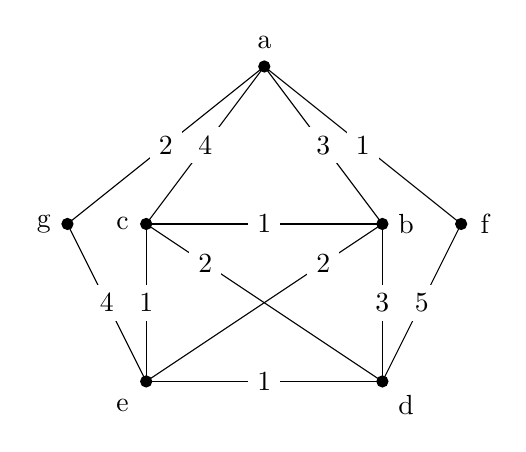
\begin{tikzpicture}

%% vertices
\draw[fill=black] (2.5,4) circle (2pt); %% a
\draw[fill=black] (4,2) circle (2pt);   %% b
\draw[fill=black] (1,2) circle (2pt);   %% c
\draw[fill=black] (4,0) circle (2pt);   %% d
\draw[fill=black] (1,0) circle (2pt);   %% e
\draw[fill=black] (5,2) circle (2pt);   %% f
\draw[fill=black] (0,2) circle (2pt);   %% g

%% vertex labels
\node at (2.5,4.3) (a){a};
\node at (4.3,2) (b){b};
\node at (0.7,2) (c){c};
\node at (4.3,-0.3) (d){d};
\node at (0.7,-0.3) (e){e};
\node at (5.3,2) (f){f};
\node at (-0.3,2) (g){g};

%%% edges
\draw (2.5,4) -- (4,2) node [midway, fill=white] {3};   %% ab
\draw (2.5,4) -- (1,2) node [midway, fill=white] {4};   %% ac
\draw (4,2) -- (1,2) node [midway, fill=white] {1};     %% bc
\draw (4,2) -- (4,0) node [midway, fill=white] {3};     %% bd
\draw (4,2) -- (1,0) node [near start, fill=white] {2}; %% be
\draw (1,2) -- (4,0) node [near start, fill=white] {2}; %% cd
\draw (1,2) -- (1,0) node [midway, fill=white] {1};     %% ce
\draw (4,0) -- (1,0) node [midway, fill=white] {1};     %% de
\draw (2.5,4) -- (5,2) node [midway, fill=white] {1};   %% af
\draw (4,0) -- (5,2) node [midway, fill=white] {5};     %% df
\draw (2.5,4) -- (0,2) node [midway, fill=white] {2};   %% ag
\draw (1,0) -- (0,2) node [midway, fill=white] {4};     %% eg
    \end{tikzpicture}
    \label{question1}
    \caption{Graph in question 1}
\end{figure}
    \include{q3(a)}
    \include{q3(b)}
    \begin{figure}
    \centering
    \begin{subfigure}[h]{0.3\textwidth}
        \centering
        \resizebox{!}{4.5cm}{
            \begin{tikzpicture}

%% vertices
\draw[fill=black] (4,6) circle (2pt);   %% a
\draw[fill=black] (3,8) circle (2pt);   %% b
\draw[fill=black] (2,6) circle (2pt);   %% c
\draw[fill=black] (6,4) circle (2pt);   %% d
\draw[fill=black] (0,4) circle (2pt);   %% e
\draw[fill=black] (4,4) circle (2pt);   %% f
\draw[fill=black] (2,4) circle (2pt);   %% g
\draw[fill=black] (4,2) circle (2pt);   %% h
\draw[fill=black] (2,2) circle (2pt);   %% i
\draw[fill=black] (4,0) circle (2pt);   %% k
\draw[fill=black] (2,0) circle (2pt);   %% l
\draw[fill=black] (0,2) circle (2pt);   %% m
\draw[fill=black] (6,2) circle (2pt);   %% n


%% vertex labels
\node at (4.3,6.3) {A};
%\node at (3,8.3) {B};
%\node at (1.7,6.3) {C};
\node at (6.3,4.3) {D};
%\node at (-0.3,4.3) {E};
%\node at (4.3,4.3) {F};
%\node at (1.7,4.3) {G};
%\node at (4.3,1.7) {H};
%\node at (1.7,1.7) {I};
%\node at (4.3,-0.3) {J};
%\node at (1.7,-0.3) {K};
%\node at (-0.3,1.7) {M};
%\node at (6.3,1.7) {N};

%%% edges
%\draw (4,6) -- (3,8) node [midway, fill=white] {1};     %% ab
%\draw (4,4) -- (2,4) node [midway, fill=white] {1};     %% fg
%\draw (4,4) -- (4,2) node [midway, fill=white] {1};     %% fh
%\draw (4,2) -- (6,2) node [midway, fill=white] {1};     %% hn
%\draw (0,4) -- (2,2) node [near start, fill=white] {1}; %% ei
%\draw (2,2) -- (2,0) node [near start, fill=white] {1}; %% il
\draw (4,6) -- (6,4) node [midway, fill=white] {2};     %% ad
%\draw (4,2) -- (2,2) node [midway, fill=white] {2};     %% hi
%\draw (2,0) -- (0,2) node [midway, fill=white] {2};     %% lm
%\draw (6,4) -- (4,2) node [midway, fill=white] {3};     %% dh
%\draw (2,6) -- (2,4) node [midway, fill=white] {3};     %% cg
%\draw (4,2) -- (4,0) node [midway, fill=white] {4};     %% hk
%\draw (6,4) -- (6,2) node [midway, fill=white] {4};     %% dn
%\draw (2,4) -- (2,2) node [midway, fill=white] {4};     %% gi
%\draw (2,6) -- (0,4) node [midway, fill=white] {5};     %% ce
%\draw (4,6) -- (4,4) node [midway, fill=white] {5};     %% af
%\draw (4,0) -- (6,2) node [near start, fill=white] {5}; %% kn
%\draw (0,4) -- (2,4) node [near start, fill=white] {6}; %% eg
%\draw (4,6) -- (2,6) node [midway, fill=white] {6};     %% ac
%\draw (3,8) -- (2,6) node [midway, fill=white] {7};     %% bc
%\draw (4,0) -- (2,0) node [midway, fill=white] {7};     %% kl
%\draw (6,4) -- (4,4) node [midway, fill=white] {7};     %% df
%\draw (2,2) -- (0,2) node [midway, fill=white] {8};     %% im
%\draw (0,4) -- (0,2) node [midway, fill=white] {9};     %% em
            \end{tikzpicture}
        }
        \label{a-d}
        \caption{Add AD}
    \end{subfigure}
    \begin{subfigure}[h]{0.3\textwidth}
        \centering
        \resizebox{!}{4.5cm}{
            \begin{tikzpicture}

%% vertices
\draw[fill=black] (4,6) circle (2pt);   %% a
\draw[fill=black] (3,8) circle (2pt);   %% b
\draw[fill=black] (2,6) circle (2pt);   %% c
\draw[fill=black] (6,4) circle (2pt);   %% d
\draw[fill=black] (0,4) circle (2pt);   %% e
\draw[fill=black] (4,4) circle (2pt);   %% f
\draw[fill=black] (2,4) circle (2pt);   %% g
\draw[fill=black] (4,2) circle (2pt);   %% h
\draw[fill=black] (2,2) circle (2pt);   %% i
\draw[fill=black] (4,0) circle (2pt);   %% k
\draw[fill=black] (2,0) circle (2pt);   %% l
\draw[fill=black] (0,2) circle (2pt);   %% m
\draw[fill=black] (6,2) circle (2pt);   %% n


%% vertex labels
\node at (4.3,6.3) {A};
\node at (3,8.3) {B};
%\node at (1.7,6.3) {C};
\node at (6.3,4.3) {D};
%\node at (-0.3,4.3) {E};
%\node at (4.3,4.3) {F};
%\node at (1.7,4.3) {G};
%\node at (4.3,1.7) {H};
%\node at (1.7,1.7) {I};
%\node at (4.3,-0.3) {J};
%\node at (1.7,-0.3) {K};
%\node at (-0.3,1.7) {M};
%\node at (6.3,1.7) {N};

%%% edges
\draw (4,6) -- (3,8) node [midway, fill=white] {1};     %% ab
%\draw (4,4) -- (2,4) node [midway, fill=white] {1};     %% fg
%\draw (4,4) -- (4,2) node [midway, fill=white] {1};     %% fh
%\draw (4,2) -- (6,2) node [midway, fill=white] {1};     %% hn
%\draw (0,4) -- (2,2) node [near start, fill=white] {1}; %% ei
%\draw (2,2) -- (2,0) node [near start, fill=white] {1}; %% il
\draw (4,6) -- (6,4) node [midway, fill=white] {2};     %% ad
%\draw (4,2) -- (2,2) node [midway, fill=white] {2};     %% hi
%\draw (2,0) -- (0,2) node [midway, fill=white] {2};     %% lm
%\draw (6,4) -- (4,2) node [midway, fill=white] {3};     %% dh
%\draw (2,6) -- (2,4) node [midway, fill=white] {3};     %% cg
%\draw (4,2) -- (4,0) node [midway, fill=white] {4};     %% hk
%\draw (6,4) -- (6,2) node [midway, fill=white] {4};     %% dn
%\draw (2,4) -- (2,2) node [midway, fill=white] {4};     %% gi
%\draw (2,6) -- (0,4) node [midway, fill=white] {5};     %% ce
%\draw (4,6) -- (4,4) node [midway, fill=white] {5};     %% af
%\draw (4,0) -- (6,2) node [near start, fill=white] {5}; %% kn
%\draw (0,4) -- (2,4) node [near start, fill=white] {6}; %% eg
%\draw (4,6) -- (2,6) node [midway, fill=white] {6};     %% ac
%\draw (3,8) -- (2,6) node [midway, fill=white] {7};     %% bc
%\draw (4,0) -- (2,0) node [midway, fill=white] {7};     %% kl
%\draw (6,4) -- (4,4) node [midway, fill=white] {7};     %% df
%\draw (2,2) -- (0,2) node [midway, fill=white] {8};     %% im
%\draw (0,4) -- (0,2) node [midway, fill=white] {9};     %% em
            \end{tikzpicture}
        }
        \label{a-b}
        \caption{Add AB}
    \end{subfigure}
    \begin{subfigure}[h]{0.3\textwidth}
        \centering
        \resizebox{!}{4.5cm}{
            \begin{tikzpicture}

%% vertices
\draw[fill=black] (4,6) circle (2pt);   %% a
\draw[fill=black] (3,8) circle (2pt);   %% b
\draw[fill=black] (2,6) circle (2pt);   %% c
\draw[fill=black] (6,4) circle (2pt);   %% d
\draw[fill=black] (0,4) circle (2pt);   %% e
\draw[fill=black] (4,4) circle (2pt);   %% f
\draw[fill=black] (2,4) circle (2pt);   %% g
\draw[fill=black] (4,2) circle (2pt);   %% h
\draw[fill=black] (2,2) circle (2pt);   %% i
\draw[fill=black] (4,0) circle (2pt);   %% k
\draw[fill=black] (2,0) circle (2pt);   %% l
\draw[fill=black] (0,2) circle (2pt);   %% m
\draw[fill=black] (6,2) circle (2pt);   %% n


%% vertex labels
\node at (4.3,6.3) {A};
\node at (3,8.3) {B};
%\node at (1.7,6.3) {C};
\node at (6.3,4.3) {D};
%\node at (-0.3,4.3) {E};
%\node at (4.3,4.3) {F};
%\node at (1.7,4.3) {G};
\node at (4.3,1.7) {H};
%\node at (1.7,1.7) {I};
%\node at (4.3,-0.3) {J};
%\node at (1.7,-0.3) {K};
%\node at (-0.3,1.7) {M};
%\node at (6.3,1.7) {N};

%%% edges
\draw (4,6) -- (3,8) node [midway, fill=white] {1};     %% ab
%\draw (4,4) -- (2,4) node [midway, fill=white] {1};     %% fg
%\draw (4,4) -- (4,2) node [midway, fill=white] {1};     %% fh
%\draw (4,2) -- (6,2) node [midway, fill=white] {1};     %% hn
%\draw (0,4) -- (2,2) node [near start, fill=white] {1}; %% ei
%\draw (2,2) -- (2,0) node [near start, fill=white] {1}; %% il
\draw (4,6) -- (6,4) node [midway, fill=white] {2};     %% ad
%\draw (4,2) -- (2,2) node [midway, fill=white] {2};     %% hi
%\draw (2,0) -- (0,2) node [midway, fill=white] {2};     %% lm
\draw (6,4) -- (4,2) node [midway, fill=white] {3};     %% dh
%\draw (2,6) -- (2,4) node [midway, fill=white] {3};     %% cg
%\draw (4,2) -- (4,0) node [midway, fill=white] {4};     %% hk
%\draw (6,4) -- (6,2) node [midway, fill=white] {4};     %% dn
%\draw (2,4) -- (2,2) node [midway, fill=white] {4};     %% gi
%\draw (2,6) -- (0,4) node [midway, fill=white] {5};     %% ce
%\draw (4,6) -- (4,4) node [midway, fill=white] {5};     %% af
%\draw (4,0) -- (6,2) node [near start, fill=white] {5}; %% kn
%\draw (0,4) -- (2,4) node [near start, fill=white] {6}; %% eg
%\draw (4,6) -- (2,6) node [midway, fill=white] {6};     %% ac
%\draw (3,8) -- (2,6) node [midway, fill=white] {7};     %% bc
%\draw (4,0) -- (2,0) node [midway, fill=white] {7};     %% kl
%\draw (6,4) -- (4,4) node [midway, fill=white] {7};     %% df
%\draw (2,2) -- (0,2) node [midway, fill=white] {8};     %% im
%\draw (0,4) -- (0,2) node [midway, fill=white] {9};     %% em
            \end{tikzpicture}
        }
        \label{d-h}
        \caption{Add DH}
    \end{subfigure}
    \begin{subfigure}[h]{0.3\textwidth}
        \centering
        \resizebox{!}{4.5cm}{
            \begin{tikzpicture}

%% vertices
\draw[fill=black] (4,6) circle (2pt);   %% a
\draw[fill=black] (3,8) circle (2pt);   %% b
\draw[fill=black] (2,6) circle (2pt);   %% c
\draw[fill=black] (6,4) circle (2pt);   %% d
\draw[fill=black] (0,4) circle (2pt);   %% e
\draw[fill=black] (4,4) circle (2pt);   %% f
\draw[fill=black] (2,4) circle (2pt);   %% g
\draw[fill=black] (4,2) circle (2pt);   %% h
\draw[fill=black] (2,2) circle (2pt);   %% i
\draw[fill=black] (4,0) circle (2pt);   %% k
\draw[fill=black] (2,0) circle (2pt);   %% l
\draw[fill=black] (0,2) circle (2pt);   %% m
\draw[fill=black] (6,2) circle (2pt);   %% n


%% vertex labels
\node at (4.3,6.3) {A};
\node at (3,8.3) {B};
%\node at (1.7,6.3) {C};
\node at (6.3,4.3) {D};
%\node at (-0.3,4.3) {E};
\node at (4.3,4.3) {F};
%\node at (1.7,4.3) {G};
\node at (4.3,1.7) {H};
%\node at (1.7,1.7) {I};
%\node at (4.3,-0.3) {J};
%\node at (1.7,-0.3) {K};
%\node at (-0.3,1.7) {M};
%\node at (6.3,1.7) {N};

%%% edges
\draw (4,6) -- (3,8) node [midway, fill=white] {1};     %% ab
%\draw (4,4) -- (2,4) node [midway, fill=white] {1};     %% fg
\draw (4,4) -- (4,2) node [midway, fill=white] {1};     %% fh
%\draw (4,2) -- (6,2) node [midway, fill=white] {1};     %% hn
%\draw (0,4) -- (2,2) node [near start, fill=white] {1}; %% ei
%\draw (2,2) -- (2,0) node [near start, fill=white] {1}; %% il
\draw (4,6) -- (6,4) node [midway, fill=white] {2};     %% ad
%\draw (4,2) -- (2,2) node [midway, fill=white] {2};     %% hi
%\draw (2,0) -- (0,2) node [midway, fill=white] {2};     %% lm
\draw (6,4) -- (4,2) node [midway, fill=white] {3};     %% dh
%\draw (2,6) -- (2,4) node [midway, fill=white] {3};     %% cg
%\draw (4,2) -- (4,0) node [midway, fill=white] {4};     %% hk
%\draw (6,4) -- (6,2) node [midway, fill=white] {4};     %% dn
%\draw (2,4) -- (2,2) node [midway, fill=white] {4};     %% gi
%\draw (2,6) -- (0,4) node [midway, fill=white] {5};     %% ce
%\draw (4,6) -- (4,4) node [midway, fill=white] {5};     %% af
%\draw (4,0) -- (6,2) node [near start, fill=white] {5}; %% kn
%\draw (0,4) -- (2,4) node [near start, fill=white] {6}; %% eg
%\draw (4,6) -- (2,6) node [midway, fill=white] {6};     %% ac
%\draw (3,8) -- (2,6) node [midway, fill=white] {7};     %% bc
%\draw (4,0) -- (2,0) node [midway, fill=white] {7};     %% kl
%\draw (6,4) -- (4,4) node [midway, fill=white] {7};     %% df
%\draw (2,2) -- (0,2) node [midway, fill=white] {8};     %% im
%\draw (0,4) -- (0,2) node [midway, fill=white] {9};     %% em
            \end{tikzpicture}
        }
        \label{f-h}
        \caption{Add FH}
    \end{subfigure}
    \begin{subfigure}[h]{0.3\textwidth}
        \centering
        \resizebox{!}{4.5cm}{
            \begin{tikzpicture}

%% vertices
\draw[fill=black] (4,6) circle (2pt);   %% a
\draw[fill=black] (3,8) circle (2pt);   %% b
\draw[fill=black] (2,6) circle (2pt);   %% c
\draw[fill=black] (6,4) circle (2pt);   %% d
\draw[fill=black] (0,4) circle (2pt);   %% e
\draw[fill=black] (4,4) circle (2pt);   %% f
\draw[fill=black] (2,4) circle (2pt);   %% g
\draw[fill=black] (4,2) circle (2pt);   %% h
\draw[fill=black] (2,2) circle (2pt);   %% i
\draw[fill=black] (4,0) circle (2pt);   %% k
\draw[fill=black] (2,0) circle (2pt);   %% l
\draw[fill=black] (0,2) circle (2pt);   %% m
\draw[fill=black] (6,2) circle (2pt);   %% n


%% vertex labels
\node at (4.3,6.3) {A};
\node at (3,8.3) {B};
%\node at (1.7,6.3) {C};
\node at (6.3,4.3) {D};
%\node at (-0.3,4.3) {E};
\node at (4.3,4.3) {F};
\node at (1.7,4.3) {G};
\node at (4.3,1.7) {H};
%\node at (1.7,1.7) {I};
%\node at (4.3,-0.3) {J};
%\node at (1.7,-0.3) {K};
%\node at (-0.3,1.7) {M};
%\node at (6.3,1.7) {N};

%%% edges
\draw (4,6) -- (3,8) node [midway, fill=white] {1};     %% ab
\draw (4,4) -- (2,4) node [midway, fill=white] {1};     %% fg
\draw (4,4) -- (4,2) node [midway, fill=white] {1};     %% fh
%\draw (4,2) -- (6,2) node [midway, fill=white] {1};     %% hn
%\draw (0,4) -- (2,2) node [near start, fill=white] {1}; %% ei
%\draw (2,2) -- (2,0) node [near start, fill=white] {1}; %% il
\draw (4,6) -- (6,4) node [midway, fill=white] {2};     %% ad
%\draw (4,2) -- (2,2) node [midway, fill=white] {2};     %% hi
%\draw (2,0) -- (0,2) node [midway, fill=white] {2};     %% lm
\draw (6,4) -- (4,2) node [midway, fill=white] {3};     %% dh
%\draw (2,6) -- (2,4) node [midway, fill=white] {3};     %% cg
%\draw (4,2) -- (4,0) node [midway, fill=white] {4};     %% hk
%\draw (6,4) -- (6,2) node [midway, fill=white] {4};     %% dn
%\draw (2,4) -- (2,2) node [midway, fill=white] {4};     %% gi
%\draw (2,6) -- (0,4) node [midway, fill=white] {5};     %% ce
%\draw (4,6) -- (4,4) node [midway, fill=white] {5};     %% af
%\draw (4,0) -- (6,2) node [near start, fill=white] {5}; %% kn
%\draw (0,4) -- (2,4) node [near start, fill=white] {6}; %% eg
%\draw (4,6) -- (2,6) node [midway, fill=white] {6};     %% ac
%\draw (3,8) -- (2,6) node [midway, fill=white] {7};     %% bc
%\draw (4,0) -- (2,0) node [midway, fill=white] {7};     %% kl
%\draw (6,4) -- (4,4) node [midway, fill=white] {7};     %% df
%\draw (2,2) -- (0,2) node [midway, fill=white] {8};     %% im
%\draw (0,4) -- (0,2) node [midway, fill=white] {9};     %% em
            \end{tikzpicture}
        }
        \label{f-g}
        \caption{Add FG}
    \end{subfigure}
    \begin{subfigure}[h]{0.3\textwidth}
        \centering
        \resizebox{!}{4.5cm}{
            \begin{tikzpicture}

%% vertices
\draw[fill=black] (4,6) circle (2pt);   %% a
\draw[fill=black] (3,8) circle (2pt);   %% b
\draw[fill=black] (2,6) circle (2pt);   %% c
\draw[fill=black] (6,4) circle (2pt);   %% d
\draw[fill=black] (0,4) circle (2pt);   %% e
\draw[fill=black] (4,4) circle (2pt);   %% f
\draw[fill=black] (2,4) circle (2pt);   %% g
\draw[fill=black] (4,2) circle (2pt);   %% h
\draw[fill=black] (2,2) circle (2pt);   %% i
\draw[fill=black] (4,0) circle (2pt);   %% k
\draw[fill=black] (2,0) circle (2pt);   %% l
\draw[fill=black] (0,2) circle (2pt);   %% m
\draw[fill=black] (6,2) circle (2pt);   %% n


%% vertex labels
\node at (4.3,6.3) {A};
\node at (3,8.3) {B};
%\node at (1.7,6.3) {C};
\node at (6.3,4.3) {D};
%\node at (-0.3,4.3) {E};
\node at (4.3,4.3) {F};
\node at (1.7,4.3) {G};
\node at (4.3,1.7) {H};
%\node at (1.7,1.7) {I};
%\node at (4.3,-0.3) {J};
%\node at (1.7,-0.3) {K};
%\node at (-0.3,1.7) {M};
\node at (6.3,1.7) {N};

%%% edges
\draw (4,6) -- (3,8) node [midway, fill=white] {1};     %% ab
\draw (4,4) -- (2,4) node [midway, fill=white] {1};     %% fg
\draw (4,4) -- (4,2) node [midway, fill=white] {1};     %% fh
\draw (4,2) -- (6,2) node [midway, fill=white] {1};     %% hn
%\draw (0,4) -- (2,2) node [near start, fill=white] {1}; %% ei
%\draw (2,2) -- (2,0) node [near start, fill=white] {1}; %% il
\draw (4,6) -- (6,4) node [midway, fill=white] {2};     %% ad
%\draw (4,2) -- (2,2) node [midway, fill=white] {2};     %% hi
%\draw (2,0) -- (0,2) node [midway, fill=white] {2};     %% lm
\draw (6,4) -- (4,2) node [midway, fill=white] {3};     %% dh
%\draw (2,6) -- (2,4) node [midway, fill=white] {3};     %% cg
%\draw (4,2) -- (4,0) node [midway, fill=white] {4};     %% hk
%\draw (6,4) -- (6,2) node [midway, fill=white] {4};     %% dn
%\draw (2,4) -- (2,2) node [midway, fill=white] {4};     %% gi
%\draw (2,6) -- (0,4) node [midway, fill=white] {5};     %% ce
%\draw (4,6) -- (4,4) node [midway, fill=white] {5};     %% af
%\draw (4,0) -- (6,2) node [near start, fill=white] {5}; %% kn
%\draw (0,4) -- (2,4) node [near start, fill=white] {6}; %% eg
%\draw (4,6) -- (2,6) node [midway, fill=white] {6};     %% ac
%\draw (3,8) -- (2,6) node [midway, fill=white] {7};     %% bc
%\draw (4,0) -- (2,0) node [midway, fill=white] {7};     %% kl
%\draw (6,4) -- (4,4) node [midway, fill=white] {7};     %% df
%\draw (2,2) -- (0,2) node [midway, fill=white] {8};     %% im
%\draw (0,4) -- (0,2) node [midway, fill=white] {9};     %% em
            \end{tikzpicture}
        }
        \label{f-g}
        \caption{Add HN}
    \end{subfigure}
    \begin{subfigure}[h]{0.3\textwidth}
        \centering
        \resizebox{!}{4.5cm}{
            \begin{tikzpicture}

%% vertices
\draw[fill=black] (4,6) circle (2pt);   %% a
\draw[fill=black] (3,8) circle (2pt);   %% b
\draw[fill=black] (2,6) circle (2pt);   %% c
\draw[fill=black] (6,4) circle (2pt);   %% d
\draw[fill=black] (0,4) circle (2pt);   %% e
\draw[fill=black] (4,4) circle (2pt);   %% f
\draw[fill=black] (2,4) circle (2pt);   %% g
\draw[fill=black] (4,2) circle (2pt);   %% h
\draw[fill=black] (2,2) circle (2pt);   %% i
\draw[fill=black] (4,0) circle (2pt);   %% k
\draw[fill=black] (2,0) circle (2pt);   %% l
\draw[fill=black] (0,2) circle (2pt);   %% m
\draw[fill=black] (6,2) circle (2pt);   %% n


%% vertex labels
\node at (4.3,6.3) {A};
\node at (3,8.3) {B};
%\node at (1.7,6.3) {C};
\node at (6.3,4.3) {D};
%\node at (-0.3,4.3) {E};
\node at (4.3,4.3) {F};
\node at (1.7,4.3) {G};
\node at (4.3,1.7) {H};
\node at (1.7,1.7) {I};
%\node at (4.3,-0.3) {J};
%\node at (1.7,-0.3) {K};
%\node at (-0.3,1.7) {M};
\node at (6.3,1.7) {N};

%%% edges
\draw (4,6) -- (3,8) node [midway, fill=white] {1};     %% ab
\draw (4,4) -- (2,4) node [midway, fill=white] {1};     %% fg
\draw (4,4) -- (4,2) node [midway, fill=white] {1};     %% fh
\draw (4,2) -- (6,2) node [midway, fill=white] {1};     %% hn
%\draw (0,4) -- (2,2) node [near start, fill=white] {1}; %% ei
%\draw (2,2) -- (2,0) node [near start, fill=white] {1}; %% il
\draw (4,6) -- (6,4) node [midway, fill=white] {2};     %% ad
\draw (4,2) -- (2,2) node [midway, fill=white] {2};     %% hi
%\draw (2,0) -- (0,2) node [midway, fill=white] {2};     %% lm
\draw (6,4) -- (4,2) node [midway, fill=white] {3};     %% dh
%\draw (2,6) -- (2,4) node [midway, fill=white] {3};     %% cg
%\draw (4,2) -- (4,0) node [midway, fill=white] {4};     %% hk
%\draw (6,4) -- (6,2) node [midway, fill=white] {4};     %% dn
%\draw (2,4) -- (2,2) node [midway, fill=white] {4};     %% gi
%\draw (2,6) -- (0,4) node [midway, fill=white] {5};     %% ce
%\draw (4,6) -- (4,4) node [midway, fill=white] {5};     %% af
%\draw (4,0) -- (6,2) node [near start, fill=white] {5}; %% kn
%\draw (0,4) -- (2,4) node [near start, fill=white] {6}; %% eg
%\draw (4,6) -- (2,6) node [midway, fill=white] {6};     %% ac
%\draw (3,8) -- (2,6) node [midway, fill=white] {7};     %% bc
%\draw (4,0) -- (2,0) node [midway, fill=white] {7};     %% kl
%\draw (6,4) -- (4,4) node [midway, fill=white] {7};     %% df
%\draw (2,2) -- (0,2) node [midway, fill=white] {8};     %% im
%\draw (0,4) -- (0,2) node [midway, fill=white] {9};     %% em
            \end{tikzpicture}
        }
        \label{f-g}
        \caption{Add HI}
    \end{subfigure}
    \begin{subfigure}[h]{0.3\textwidth}
        \centering
        \resizebox{!}{4.5cm}{
            \begin{tikzpicture}

%% vertices
\draw[fill=black] (4,6) circle (2pt);   %% a
\draw[fill=black] (3,8) circle (2pt);   %% b
\draw[fill=black] (2,6) circle (2pt);   %% c
\draw[fill=black] (6,4) circle (2pt);   %% d
\draw[fill=black] (0,4) circle (2pt);   %% e
\draw[fill=black] (4,4) circle (2pt);   %% f
\draw[fill=black] (2,4) circle (2pt);   %% g
\draw[fill=black] (4,2) circle (2pt);   %% h
\draw[fill=black] (2,2) circle (2pt);   %% i
\draw[fill=black] (4,0) circle (2pt);   %% k
\draw[fill=black] (2,0) circle (2pt);   %% l
\draw[fill=black] (0,2) circle (2pt);   %% m
\draw[fill=black] (6,2) circle (2pt);   %% n


%% vertex labels
\node at (4.3,6.3) {A};
\node at (3,8.3) {B};
%\node at (1.7,6.3) {C};
\node at (6.3,4.3) {D};
\node at (-0.3,4.3) {E};
\node at (4.3,4.3) {F};
\node at (1.7,4.3) {G};
\node at (4.3,1.7) {H};
\node at (1.7,1.7) {I};
%\node at (4.3,-0.3) {J};
%\node at (1.7,-0.3) {K};
%\node at (-0.3,1.7) {M};
\node at (6.3,1.7) {N};

%%% edges
\draw (4,6) -- (3,8) node [midway, fill=white] {1};     %% ab
\draw (4,4) -- (2,4) node [midway, fill=white] {1};     %% fg
\draw (4,4) -- (4,2) node [midway, fill=white] {1};     %% fh
\draw (4,2) -- (6,2) node [midway, fill=white] {1};     %% hn
\draw (0,4) -- (2,2) node [near start, fill=white] {1}; %% ei
%\draw (2,2) -- (2,0) node [near start, fill=white] {1}; %% il
\draw (4,6) -- (6,4) node [midway, fill=white] {2};     %% ad
\draw (4,2) -- (2,2) node [midway, fill=white] {2};     %% hi
%\draw (2,0) -- (0,2) node [midway, fill=white] {2};     %% lm
\draw (6,4) -- (4,2) node [midway, fill=white] {3};     %% dh
%\draw (2,6) -- (2,4) node [midway, fill=white] {3};     %% cg
%\draw (4,2) -- (4,0) node [midway, fill=white] {4};     %% hk
%\draw (6,4) -- (6,2) node [midway, fill=white] {4};     %% dn
%\draw (2,4) -- (2,2) node [midway, fill=white] {4};     %% gi
%\draw (2,6) -- (0,4) node [midway, fill=white] {5};     %% ce
%\draw (4,6) -- (4,4) node [midway, fill=white] {5};     %% af
%\draw (4,0) -- (6,2) node [near start, fill=white] {5}; %% kn
%\draw (0,4) -- (2,4) node [near start, fill=white] {6}; %% eg
%\draw (4,6) -- (2,6) node [midway, fill=white] {6};     %% ac
%\draw (3,8) -- (2,6) node [midway, fill=white] {7};     %% bc
%\draw (4,0) -- (2,0) node [midway, fill=white] {7};     %% kl
%\draw (6,4) -- (4,4) node [midway, fill=white] {7};     %% df
%\draw (2,2) -- (0,2) node [midway, fill=white] {8};     %% im
%\draw (0,4) -- (0,2) node [midway, fill=white] {9};     %% em
            \end{tikzpicture}
        }
        \label{f-g}
        \caption{Add EI}
    \end{subfigure}
    \begin{subfigure}[h]{0.3\textwidth}
        \centering
        \resizebox{!}{4.5cm}{
            \begin{tikzpicture}

%% vertices
\draw[fill=black] (4,6) circle (2pt);   %% a
\draw[fill=black] (3,8) circle (2pt);   %% b
\draw[fill=black] (2,6) circle (2pt);   %% c
\draw[fill=black] (6,4) circle (2pt);   %% d
\draw[fill=black] (0,4) circle (2pt);   %% e
\draw[fill=black] (4,4) circle (2pt);   %% f
\draw[fill=black] (2,4) circle (2pt);   %% g
\draw[fill=black] (4,2) circle (2pt);   %% h
\draw[fill=black] (2,2) circle (2pt);   %% i
\draw[fill=black] (4,0) circle (2pt);   %% k
\draw[fill=black] (2,0) circle (2pt);   %% l
\draw[fill=black] (0,2) circle (2pt);   %% m
\draw[fill=black] (6,2) circle (2pt);   %% n


%% vertex labels
\node at (4.3,6.3) {A};
\node at (3,8.3) {B};
%\node at (1.7,6.3) {C};
\node at (6.3,4.3) {D};
\node at (-0.3,4.3) {E};
\node at (4.3,4.3) {F};
\node at (1.7,4.3) {G};
\node at (4.3,1.7) {H};
\node at (1.7,1.7) {I};
%\node at (4.3,-0.3) {J};
%\node at (1.7,-0.3) {K};
\node at (1.7,-0.3) {L};
%\node at (-0.3,1.7) {M};
\node at (6.3,1.7) {N};

%%% edges
\draw (4,6) -- (3,8) node [midway, fill=white] {1};     %% ab
\draw (4,4) -- (2,4) node [midway, fill=white] {1};     %% fg
\draw (4,4) -- (4,2) node [midway, fill=white] {1};     %% fh
\draw (4,2) -- (6,2) node [midway, fill=white] {1};     %% hn
\draw (0,4) -- (2,2) node [near start, fill=white] {1}; %% ei
\draw (2,2) -- (2,0) node [near start, fill=white] {1}; %% il
\draw (4,6) -- (6,4) node [midway, fill=white] {2};     %% ad
\draw (4,2) -- (2,2) node [midway, fill=white] {2};     %% hi
%\draw (2,0) -- (0,2) node [midway, fill=white] {2};     %% lm
\draw (6,4) -- (4,2) node [midway, fill=white] {3};     %% dh
%\draw (2,6) -- (2,4) node [midway, fill=white] {3};     %% cg
%\draw (4,2) -- (4,0) node [midway, fill=white] {4};     %% hk
%\draw (6,4) -- (6,2) node [midway, fill=white] {4};     %% dn
%\draw (2,4) -- (2,2) node [midway, fill=white] {4};     %% gi
%\draw (2,6) -- (0,4) node [midway, fill=white] {5};     %% ce
%\draw (4,6) -- (4,4) node [midway, fill=white] {5};     %% af
%\draw (4,0) -- (6,2) node [near start, fill=white] {5}; %% kn
%\draw (0,4) -- (2,4) node [near start, fill=white] {6}; %% eg
%\draw (4,6) -- (2,6) node [midway, fill=white] {6};     %% ac
%\draw (3,8) -- (2,6) node [midway, fill=white] {7};     %% bc
%\draw (4,0) -- (2,0) node [midway, fill=white] {7};     %% kl
%\draw (6,4) -- (4,4) node [midway, fill=white] {7};     %% df
%\draw (2,2) -- (0,2) node [midway, fill=white] {8};     %% im
%\draw (0,4) -- (0,2) node [midway, fill=white] {9};     %% em
            \end{tikzpicture}
        }
        \label{f-g}
        \caption{Add IL}
    \end{subfigure}
    \begin{subfigure}[h]{0.3\textwidth}
        \centering
        \resizebox{!}{4.5cm}{
            \begin{tikzpicture}

%% vertices
\draw[fill=black] (4,6) circle (2pt);   %% a
\draw[fill=black] (3,8) circle (2pt);   %% b
\draw[fill=black] (2,6) circle (2pt);   %% c
\draw[fill=black] (6,4) circle (2pt);   %% d
\draw[fill=black] (0,4) circle (2pt);   %% e
\draw[fill=black] (4,4) circle (2pt);   %% f
\draw[fill=black] (2,4) circle (2pt);   %% g
\draw[fill=black] (4,2) circle (2pt);   %% h
\draw[fill=black] (2,2) circle (2pt);   %% i
\draw[fill=black] (4,0) circle (2pt);   %% k
\draw[fill=black] (2,0) circle (2pt);   %% l
\draw[fill=black] (0,2) circle (2pt);   %% m
\draw[fill=black] (6,2) circle (2pt);   %% n


%% vertex labels
\node at (4.3,6.3) {A};
\node at (3,8.3) {B};
%\node at (1.7,6.3) {C};
\node at (6.3,4.3) {D};
\node at (-0.3,4.3) {E};
\node at (4.3,4.3) {F};
\node at (1.7,4.3) {G};
\node at (4.3,1.7) {H};
\node at (1.7,1.7) {I};
%\node at (4.3,-0.3) {J};
%\node at (1.7,-0.3) {K};
\node at (1.7,-0.3) {L};
\node at (-0.3,1.7) {M};
\node at (6.3,1.7) {N};

%%% edges
\draw (4,6) -- (3,8) node [midway, fill=white] {1};     %% ab
\draw (4,4) -- (2,4) node [midway, fill=white] {1};     %% fg
\draw (4,4) -- (4,2) node [midway, fill=white] {1};     %% fh
\draw (4,2) -- (6,2) node [midway, fill=white] {1};     %% hn
\draw (0,4) -- (2,2) node [near start, fill=white] {1}; %% ei
\draw (2,2) -- (2,0) node [near start, fill=white] {1}; %% il
\draw (4,6) -- (6,4) node [midway, fill=white] {2};     %% ad
\draw (4,2) -- (2,2) node [midway, fill=white] {2};     %% hi
\draw (2,0) -- (0,2) node [midway, fill=white] {2};     %% lm
\draw (6,4) -- (4,2) node [midway, fill=white] {3};     %% dh
%\draw (2,6) -- (2,4) node [midway, fill=white] {3};     %% cg
%\draw (4,2) -- (4,0) node [midway, fill=white] {4};     %% hk
%\draw (6,4) -- (6,2) node [midway, fill=white] {4};     %% dn
%\draw (2,4) -- (2,2) node [midway, fill=white] {4};     %% gi
%\draw (2,6) -- (0,4) node [midway, fill=white] {5};     %% ce
%\draw (4,6) -- (4,4) node [midway, fill=white] {5};     %% af
%\draw (4,0) -- (6,2) node [near start, fill=white] {5}; %% kn
%\draw (0,4) -- (2,4) node [near start, fill=white] {6}; %% eg
%\draw (4,6) -- (2,6) node [midway, fill=white] {6};     %% ac
%\draw (3,8) -- (2,6) node [midway, fill=white] {7};     %% bc
%\draw (4,0) -- (2,0) node [midway, fill=white] {7};     %% kl
%\draw (6,4) -- (4,4) node [midway, fill=white] {7};     %% df
%\draw (2,2) -- (0,2) node [midway, fill=white] {8};     %% im
%\draw (0,4) -- (0,2) node [midway, fill=white] {9};     %% em
            \end{tikzpicture}
        }
        \label{f-g}
        \caption{Add LM}
    \end{subfigure}
    \begin{subfigure}[h]{0.3\textwidth}
        \centering
        \resizebox{!}{4.5cm}{
            \begin{tikzpicture}

%% vertices
\draw[fill=black] (4,6) circle (2pt);   %% a
\draw[fill=black] (3,8) circle (2pt);   %% b
\draw[fill=black] (2,6) circle (2pt);   %% c
\draw[fill=black] (6,4) circle (2pt);   %% d
\draw[fill=black] (0,4) circle (2pt);   %% e
\draw[fill=black] (4,4) circle (2pt);   %% f
\draw[fill=black] (2,4) circle (2pt);   %% g
\draw[fill=black] (4,2) circle (2pt);   %% h
\draw[fill=black] (2,2) circle (2pt);   %% i
\draw[fill=black] (4,0) circle (2pt);   %% k
\draw[fill=black] (2,0) circle (2pt);   %% l
\draw[fill=black] (0,2) circle (2pt);   %% m
\draw[fill=black] (6,2) circle (2pt);   %% n


%% vertex labels
\node at (4.3,6.3) {A};
\node at (3,8.3) {B};
\node at (1.7,6.3) {C};
\node at (6.3,4.3) {D};
\node at (-0.3,4.3) {E};
\node at (4.3,4.3) {F};
\node at (1.7,4.3) {G};
\node at (4.3,1.7) {H};
\node at (1.7,1.7) {I};
%\node at (4.3,-0.3) {K};
\node at (1.7,-0.3) {L};
\node at (-0.3,1.7) {M};
\node at (6.3,1.7) {N};

%%% edges
\draw (4,6) -- (3,8) node [midway, fill=white] {1};     %% ab
\draw (4,4) -- (2,4) node [midway, fill=white] {1};     %% fg
\draw (4,4) -- (4,2) node [midway, fill=white] {1};     %% fh
\draw (4,2) -- (6,2) node [midway, fill=white] {1};     %% hn
\draw (0,4) -- (2,2) node [near start, fill=white] {1}; %% ei
\draw (2,2) -- (2,0) node [near start, fill=white] {1}; %% il
\draw (4,6) -- (6,4) node [midway, fill=white] {2};     %% ad
\draw (4,2) -- (2,2) node [midway, fill=white] {2};     %% hi
\draw (2,0) -- (0,2) node [midway, fill=white] {2};     %% lm
\draw (6,4) -- (4,2) node [midway, fill=white] {3};     %% dh
\draw (2,6) -- (2,4) node [midway, fill=white] {3};     %% cg
%\draw (4,2) -- (4,0) node [midway, fill=white] {4};     %% hk
%\draw (6,4) -- (6,2) node [midway, fill=white] {4};     %% dn
%\draw (2,4) -- (2,2) node [midway, fill=white] {4};     %% gi
%\draw (2,6) -- (0,4) node [midway, fill=white] {5};     %% ce
%\draw (4,6) -- (4,4) node [midway, fill=white] {5};     %% af
%\draw (4,0) -- (6,2) node [near start, fill=white] {5}; %% kn
%\draw (0,4) -- (2,4) node [near start, fill=white] {6}; %% eg
%\draw (4,6) -- (2,6) node [midway, fill=white] {6};     %% ac
%\draw (3,8) -- (2,6) node [midway, fill=white] {7};     %% bc
%\draw (4,0) -- (2,0) node [midway, fill=white] {7};     %% kl
%\draw (6,4) -- (4,4) node [midway, fill=white] {7};     %% df
%\draw (2,2) -- (0,2) node [midway, fill=white] {8};     %% im
%\draw (0,4) -- (0,2) node [midway, fill=white] {9};     %% em
            \end{tikzpicture}
        }
        \label{f-g}
        \caption{Add CG}
    \end{subfigure}
    \begin{subfigure}[h]{0.3\textwidth}
        \centering
        \resizebox{!}{4.5cm}{
            \begin{tikzpicture}

%% vertices
\draw[fill=black] (4,6) circle (2pt);   %% a
\draw[fill=black] (3,8) circle (2pt);   %% b
\draw[fill=black] (2,6) circle (2pt);   %% c
\draw[fill=black] (6,4) circle (2pt);   %% d
\draw[fill=black] (0,4) circle (2pt);   %% e
\draw[fill=black] (4,4) circle (2pt);   %% f
\draw[fill=black] (2,4) circle (2pt);   %% g
\draw[fill=black] (4,2) circle (2pt);   %% h
\draw[fill=black] (2,2) circle (2pt);   %% i
\draw[fill=black] (4,0) circle (2pt);   %% k
\draw[fill=black] (2,0) circle (2pt);   %% l
\draw[fill=black] (0,2) circle (2pt);   %% m
\draw[fill=black] (6,2) circle (2pt);   %% n


%% vertex labels
\node at (4.3,6.3) {A};
\node at (3,8.3) {B};
\node at (1.7,6.3) {C};
\node at (6.3,4.3) {D};
\node at (-0.3,4.3) {E};
\node at (4.3,4.3) {F};
\node at (1.7,4.3) {G};
\node at (4.3,1.7) {H};
\node at (1.7,1.7) {I};
\node at (4.3,-0.3) {K};
\node at (1.7,-0.3) {L};
\node at (-0.3,1.7) {M};
\node at (6.3,1.7) {N};

%%% edges
\draw (4,6) -- (3,8) node [midway, fill=white] {1};     %% ab
\draw (4,4) -- (2,4) node [midway, fill=white] {1};     %% fg
\draw (4,4) -- (4,2) node [midway, fill=white] {1};     %% fh
\draw (4,2) -- (6,2) node [midway, fill=white] {1};     %% hn
\draw (0,4) -- (2,2) node [near start, fill=white] {1}; %% ei
\draw (2,2) -- (2,0) node [near start, fill=white] {1}; %% il
\draw (4,6) -- (6,4) node [midway, fill=white] {2};     %% ad
\draw (4,2) -- (2,2) node [midway, fill=white] {2};     %% hi
\draw (2,0) -- (0,2) node [midway, fill=white] {2};     %% lm
\draw (6,4) -- (4,2) node [midway, fill=white] {3};     %% dh
\draw (2,6) -- (2,4) node [midway, fill=white] {3};     %% cg
\draw (4,2) -- (4,0) node [midway, fill=white] {4};     %% hk
%\draw (6,4) -- (6,2) node [midway, fill=white] {4};     %% dn
%\draw (2,4) -- (2,2) node [midway, fill=white] {4};     %% gi
%\draw (2,6) -- (0,4) node [midway, fill=white] {5};     %% ce
%\draw (4,6) -- (4,4) node [midway, fill=white] {5};     %% af
%\draw (4,0) -- (6,2) node [near start, fill=white] {5}; %% kn
%\draw (0,4) -- (2,4) node [near start, fill=white] {6}; %% eg
%\draw (4,6) -- (2,6) node [midway, fill=white] {6};     %% ac
%\draw (3,8) -- (2,6) node [midway, fill=white] {7};     %% bc
%\draw (4,0) -- (2,0) node [midway, fill=white] {7};     %% kl
%\draw (6,4) -- (4,4) node [midway, fill=white] {7};     %% df
%\draw (2,2) -- (0,2) node [midway, fill=white] {8};     %% im
%\draw (0,4) -- (0,2) node [midway, fill=white] {9};     %% em
            \end{tikzpicture}
        }
        \label{f-g}
        \caption{Add HK}
    \end{subfigure}
    \caption{Spanning tree using Prim's algorithm}
    \label{prim}
\end{figure}
    \include{q4(a)}
    \begin{figure}
    \centering
    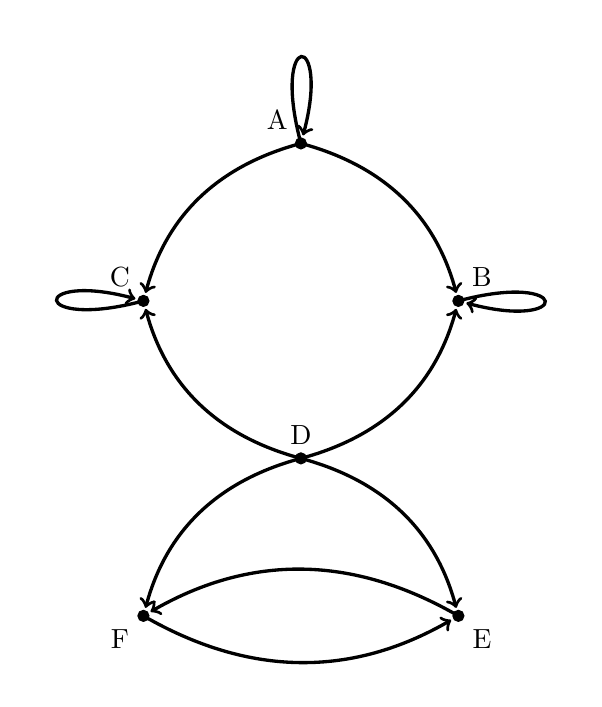
\begin{tikzpicture}

%% vertices
\draw[fill=black] (2,6) circle (2pt);   %% a
\draw[fill=black] (0,4) circle (2pt);   %% b
\draw[fill=black] (4,4) circle (2pt);   %% c
\draw[fill=black] (2,2) circle (2pt);   %% d
\draw[fill=black] (0,0) circle (2pt);   %% e
\draw[fill=black] (4,0) circle (2pt);   %% f

%% vertex labels
\node at (1.7,6.3) {A};
\node at (-0.3,4.3) {C};
\node at (4.3,4.3) {B};
\node at (2,2.3) {D};
\node at (-0.3,-0.3) {F};
\node at (4.3,-0.3) {E};

%%% edges
\draw[-{>[sep=3pt]}, very thick] (2,6) to [loop above, min distance=1.5cm] (2,6);     %% aa
\draw[-{>[sep=3pt]}, very thick] (2,6) to [bend right] (0,4);     %% ab
\draw[-{>[sep=3pt]}, very thick] (0,4) to [loop left, min distance=1.5cm] (0,4);     %% bb
\draw[-{>[sep=3pt]}, very thick] (2,6) to [bend left] (4,4);     %% ac
\draw[-{>[sep=3pt]}, very thick] (4,4) to [loop right, min distance=1.5cm] (4,4); %% cc
\draw[-{>[sep=3pt]}, very thick] (2,2) to [bend right] (4,4); %% dc
\draw[-{>[sep=3pt]}, very thick] (2,2) to [bend left] (0,4);     %% db
\draw[-{>[sep=3pt]}, very thick] (2,2) to [bend right] (0,0);     %% de
\draw[-{>[sep=3pt]}, very thick] (2,2) to [bend left] (4,0);     %% df
\draw[-{>[sep=3pt]}, very thick] (0,0) to [bend right] (4,0);     %% ef
\draw[-{>[sep=3pt]}, very thick] (4,0) to [bend right] (0,0);     %% fe
    \end{tikzpicture}
    \label{q4-a}
    \caption{Isomorphism in quesrtion 4}
\end{figure}
    \include{q5(a)}
    \begin{figure}
    \centering
    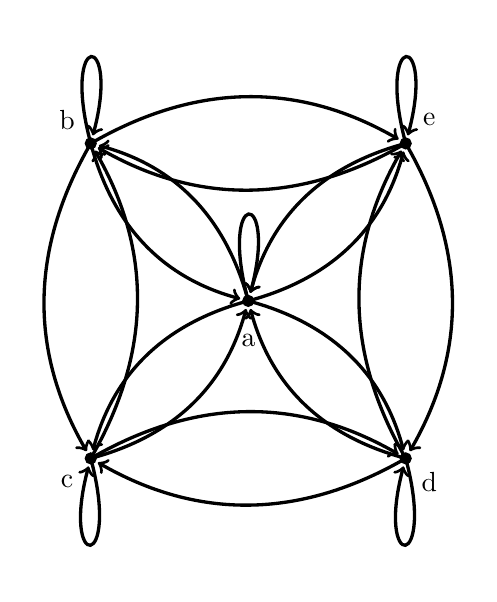
\begin{tikzpicture}

%% vertices
\draw[fill=black] (2,2) circle (2pt);   %% a
\draw[fill=black] (0,4) circle (2pt);   %% b
\draw[fill=black] (0,0) circle (2pt);   %% c
\draw[fill=black] (4,0) circle (2pt);   %% d
\draw[fill=black] (4,4) circle (2pt);   %% e

%% vertex labels
\node at (2,1.5) {a};
\node at (-0.3,4.3) {b};
\node at (-0.3,-0.3) {c};
\node at (4.3,-0.3) {d};
\node at (4.3,4.3) {e};

%%% edges
\draw[-{>[sep=3pt]}, very thick] (2,2) to [loop above, min distance=1.5cm] (2,2);     %% aa
\draw[-{>[sep=3pt]}, very thick] (2,2) to [bend right] (0,4);     %% ab
\draw[-{>[sep=3pt]}, very thick] (0,4) to [bend right] (2,2);     %% ba
\draw[-{>[sep=3pt]}, very thick] (0,4) to [loop above, min distance=1.5cm] (0,4);     %% bb
\draw[-{>[sep=3pt]}, very thick] (2,2) to [bend right] (4,4); %% ae
\draw[-{>[sep=3pt]}, very thick] (4,4) to [bend right] (2,2); %% ea
\draw[-{>[sep=3pt]}, very thick] (4,4) to [loop above, min distance=1.5cm] (4,4);     %% ee
\draw[-{>[sep=3pt]}, very thick] (2,2) to [bend right] (0,0);     %% ac
\draw[-{>[sep=3pt]}, very thick] (2,2) to [bend left] (4,0);     %% ad
\draw[-{>[sep=3pt]}, very thick] (0,4) to [bend right] (0,0);     %% bc
\draw[-{>[sep=3pt]}, very thick] (4,4) to [bend left] (4,0);     %% ed
\draw[-{>[sep=3pt]}, very thick] (0,0) to [loop below, min distance=1.5cm] (0,0);%%cc
\draw[-{>[sep=3pt]}, very thick] (4,0) to [loop below, min distance=1.5cm] (4,0);%%dd
\draw[-{>[sep=3pt]}, very thick] (0,0) to [bend right] (2,2);%%ca
\draw[-{>[sep=3pt]}, very thick] (4,0) to [bend left] (2,2);%%da
\draw[-{>[sep=3pt]}, very thick] (0,0) to [bend right] (0,4);%%cb
\draw[-{>[sep=3pt]}, very thick] (4,0) to [bend left] (4,4);%%de
\draw[-{>[sep=3pt]}, very thick] (0,4) to [bend left] (4,4);%%be
\draw[-{>[sep=3pt]}, very thick] (4,4) to [bend left] (0,4);%%eb
\draw[-{>[sep=3pt]}, very thick] (0,0) to [bend left] (4,0);%%cd
\draw[-{>[sep=3pt]}, very thick] (4,0) to [bend left] (0,0);%%dc
    \end{tikzpicture}
    \label{q4-a}
    \caption{Reflexive relation}
\end{figure}
\end{document}